132. \begin{figure}[ht!]
\center{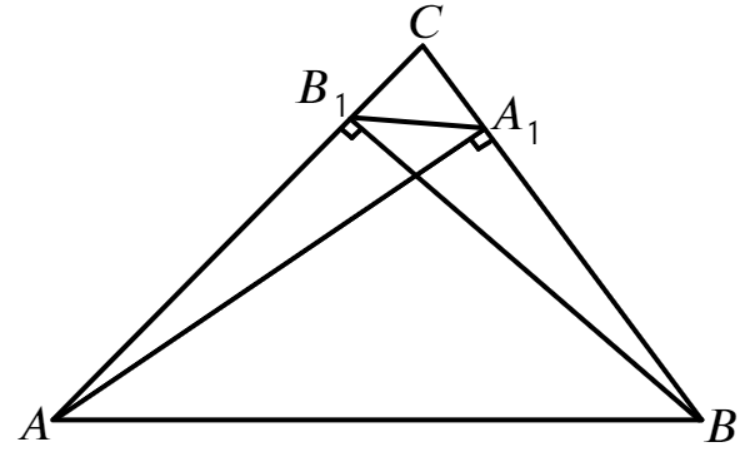
\includegraphics[scale=0.35]{g8-131.png}}
\end{figure}\\
В четырёхугольнике $AB_1A_1B$ угол, образованный стороной $AB_1$ и диагональю $BB_1,$ равен углу, образованному стороной $BA_1$ и диагональю $AA_1,$ значит он является вписанным. Тогда $\angle A_1B_1A+\angle CBA=180^\circ,\ \angle A_1B_1A=180^\circ-17^\circ=163^\circ.$ Угол $\angle CB_1A_1$ является смежным к нему, значит $\angle CB_1A_1=180^\circ-163^\circ=17^\circ.$\\
